\chapter{Optimizadores para la gradiente de descenso en una Red Neuronal Convolucional}
En este capítulo se detallarán algunos algoritmos de optimización de Aprendizaje automático y principalmente se enfocará en aquellos que serán utilizados en nuestra red neuronal convolucional.\\
Al inicio de este capítulo veremos una introducción a este tipo de redes de prealimentación.

\section{Redes Neuronales Convolucionales}
Las CNN son un tipo de redes neuronales especiales para procesar datos como imágenes las cuales son más difíciles de tratar en una red neuronal tradicional, como por ejemplo en el caso del perceptron multicapas.\\ El término \textit{convolucional} hace referencia a la operación lineal matemática usada. Las redes neuronales convolucionales usan esta operación para aprender de las características de mayor orden presente en los datos.
La primera CNN fue creada por Yann LeCun. Entre sus usos más comunes tenemos el reconocimiento de imágenes y lenguaje natural.\\
Las redes neuronales convolucionales fueron inspiradas en la corteza visuales de los animales. Las células de la corteza visual, estas se activan para realizar tareas como el reconocimiento de patrones.

\subsection{Estructura de una imagen}
Debido a que las redes neuronales convolucionales trabajan principalmente con imágenes, es importante conocer cual es la estructura de una imagen y cómo es que la computadora comprende y utiliza esta información.\\
Las imágenes están constituidas por una sucesión de píxeles, podemos entender el pixel como la menor unidad homogénea en color de una imagen digital. Teniendo este concepto, podemos dividir la información de una imagen de la siguiente forma:
\begin{itemize}
	\item \textbf{Width}: El ancho de la imagen medido en pixeles
	\item \textbf{Height}: El alto de la imagen medida en pixeles.
	\item \textbf{Canales RGB}: Estos canales contiene la información de los colores y profundidad de una imagen. Este canal guarda la información en tres canales Red, Green y Blue.
\end{itemize}

\begin{figure}[H]
	\centering
	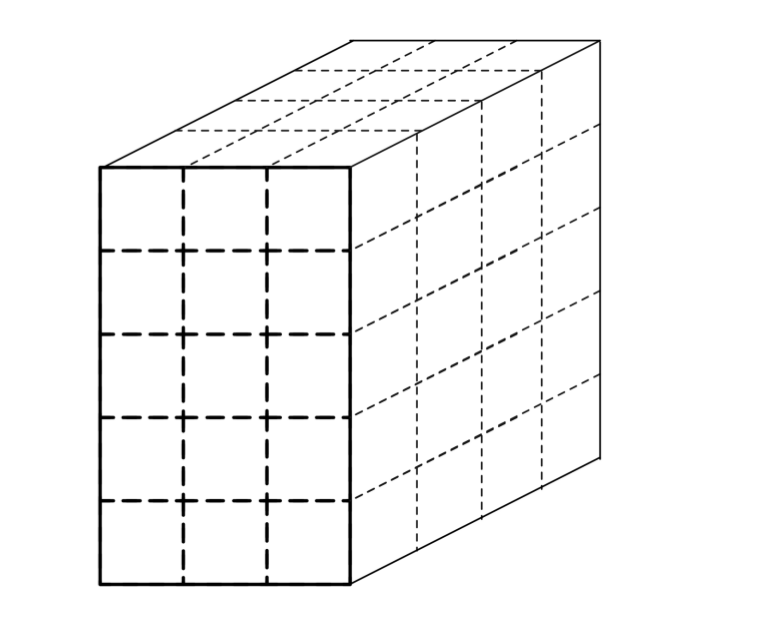
\includegraphics[width=0.7\textwidth]{Figures/image.png}
	\caption{Estructura de la imagen de entrada \\ Fuente:  \href{https://www.safaribooksonline.com/library/view/deep-learning/9781491924570/ch04.html}{\textit{Deep Learning by Adam Gibson, Josh Patterson}}}
	\label{image}
\end{figure} 

Teniendo en cuenta esta forma de guardar una podemos resaltar la ventaja de usar Redes convolucionales en lugar de usar una red neuronal multicapas.\\ Las redes multicapas toman un vector de una dimensión como entrada, si quisiéramos entrenar un perceptron multicapas con imágenes de 32x32 píxeles y con 3 canales RGB necesitaríamos crear 3072 pesos ($w_{i}$) para una sola neurona en la capa oculta. Esta generación excesiva de peso hace que la tarea resulte complicada usando redes multicapas.\\ De esta forma surge la idea de recurrir a un tiempo tipo de redes neuronales que faciliten la tarea sin consumir muchos recursos.
\subsection{Capas de una CNN}
Las redes neuronales convoluciones pueden ser dividas en distintas capas, cada una con una tarea específica para el tratamiento de la información. En esta sección describiremos cada una de estas capas.
\subsubsection{Input layer}
Esta capa es la encargada de cargar y almacenar la información de las imágenes para luego procesarlas en la red. Esta información contiene detalles de ancho, alto en píxeles y el número de canales de imagen. Las entradas de esta capa corresponden a la imagen vista en la figura 4.1.

\subsubsection{Convolutional layers}
Es una de las capas más importante en el diseño de las CNNs, esta capa es la encargada de transformar la entrada(imagen o convolución anterior) usando las conexiones de las neuronas en capas anteriores. La capa calculará el producto punto entre la región de las neuronas de la capa de entrada y los pesos a los que están colocados localmente en la capa de salida. Esta salida tendrá la misma dimensión de espacios o una dimensión menor.

Para entender más a fondo esta capa debemos definir la operación de \textit{convolución}.  La \textit{convolución} es una operación matemática que describe una regla de como fusionar 2 conjuntos de información.\textquotedblleft Esta operación tiene importancia en campos como la matemática y la física debido que permite definir un puente entre el domino del espacio/tiempo y el dominio de la frecuencias a través del uso de la transformada de fourier.\\
La convolución toma la entrada, aplica un kernel de convolución y nos da un mapa de características como salida \textquotedblright \cite{book1} .\\
Las convoluciones son usadas principalmente como un detectores de características cuyas entradas son la capa de entrada u otra convolución.
En la figura 4.2 observamos la operación de convolución que por medio del uso de un kernel o filtro de convolución extrae características de la imagen, por ejemplo detalles como bordes de una imagen.\\ Haciendo analogía con los pesos en las redes neuronales convencionales, las redes poseen el \textit{ filtro o kernel }, esto resulta beneficioso, ya que no se tendrá definir un peso para cada neurona.\\ En la figura 4.2 vemos como se aplica el kernel para producir datos de característica, este kernel será desplazado a lo largo de las dimensiones espaciales. En el desplazamiento el kernel se multiplicará por los datos de entrada dentro de su limite, produciendo una sola salida al mapa de características.
\begin{figure}[H]
	\centering
	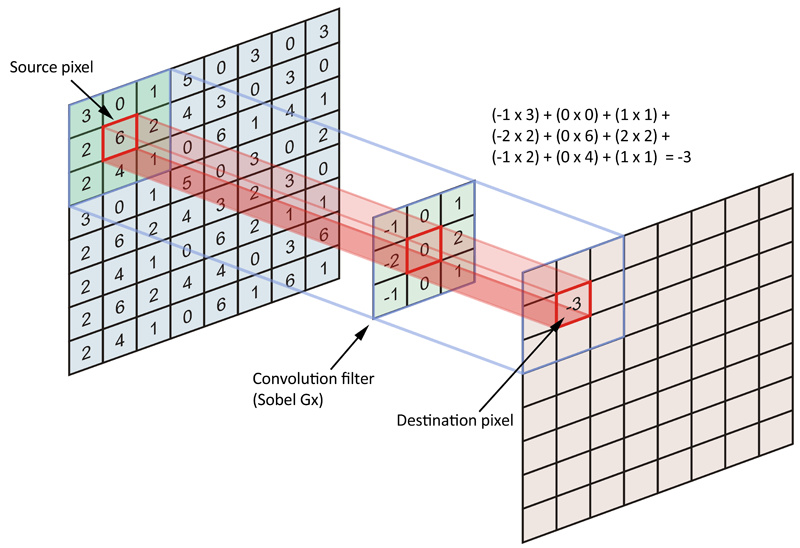
\includegraphics[width=0.7\textwidth]{Figures/convolucion.jpeg}
	\caption{Operacion de convolución \\ Fuente:  \href{http://openresearch.ai/t/network-in-network/39}{\textit{www.openresearch.ai}}}
	\label{convolucion}
\end{figure} 

Las capas convolucionales aplican transformaciones o funciones de activación al conjunto de entrada, luego el mapa de activación generado se apilará a lo largo de dimensión de profundidad para construir el volumen de salida.

\textbf{Componentes de la capa de convolución}.\\	
Las capas convolucionales poseen parámetros e hiperparámetros. La gradiente de descenso tiene la funcion de entrenar los parámetros de modo que las clases sean consistentes con las etiquetas en el conjunto de entrenamiento. Entre estos parámetros tenemos:
\textbf{Filtros}

Los filtros son una función que posee ancho(width) y alto (height) más pequeños que la entrada. Los filtros son aplicados a través de  del ancho y alto de la entrada, pero también pueden ser aplicados a lo largo de la profundidad.

\textbf{Hiperparámetros de una capa de convolución}.\\
A continuación veremos algunos hiperparámetros que determinan la disposición espacial y tamaño del volumen de salida de una capa convolucional.
\begin{itemize}
	\item \textbf{Filter size:} Cada filtro es pequeño con respecto al ancho(width) y alto(height) del la capa anterior. Por ejemplo podemos tener un filtro de tamaño $[5x5x3]$, lo representa 5 de ancho x 5 de alto x 3 de los canales RGB.
	\item \textbf{Output depth:} Este hiperparámetro controla el número de neuronas en la capa convolucional que están conectadas al mismo del volumen de entrada. Este parámetro puede ser elegido manualmente.
	\item \textbf{Stride:} Se encarga de configurar el tamaño de desplazamiento de la ventana de filtro. Cada filtro aplicado a la columna de entrada asignará más profundidad en el volumen de salida. Un stride grande creará un volumen de salida más grande y uno valor pequeño obtendrá un volumen menor.
	\item \textbf{Zero-padding:} Con este parámetro se puede controlar el volumen de salida. Es usado para mantener el tamaño espacial de entrada en la salida. 
\end{itemize}

\subsubsection{Pooling layers}
Este tipo de capas se encuentran entre las capas convolucionales. Se encarga de reducir el tamaño espacial(ancho,alto) de los datos de representación. Esta capa reduce la representación de los datos progresivamente a través de la red y ayuda a controlar el \textit{overfitting}.\\
Esta capa utiliza la operación \textit{max()} para cambiar el tamaño de los datos de entrada espacialmente, a esta operación se le conoce como max pooling. Esta funciona de siguiente forma toma un filtro de $n x n$, y la operación $max$ toma el mayor de los números en el área de filtro.\\ Por ejemplo en caso tener una imagen de entrada $32 \times 32$ píxeles y se aplica un filtro de $2\times2$, como resultado obtendremos una salida de $16\times16$ píxeles. Esto reduce cada segmento de profundidad en el volumen de entrada por un factor de 2.

\subsubsection{Fully Connected Layers}

Esta capa se calcula el puntaje de las clases que usaremos como salida de red, esta será la encargada de reconocer a que clase pertenece una imagen de prueba de acuerdo a su puntaje o probabilidad. Las dimensiones del volumen de la salida son [1x1xN], donde el valor de N corresponde al número de clases de salida que se están evaluando. En el caso del MNIST (dataset para reconocimiento de dígitos), el valor de N es igual a 10, número que corresponde a los 10 dígitos distintos que posee el dataset($0, ... ,9$).\\
Esta capa tiene conexión entre todas sus neuronas y las de la capa anterior. Esta capa realiza las transformaciones del volumen de datos de entrada. Estas son funciones de activación en el volumen de entrada y los parámetros (pesos y bias de las neuronas).
\vspace{2cm}
\subsection{Arquitecturas conocidas}
Actualmente existen algunas arquitecturas de CNN ya diseñadas que son aplicadas para el trabajo de reconocimiento de imágenes.\\ El proyecto ImageNet, posee una gran base de datos de imágenes. Este proyecto realizá una competición llamada \textit{ImageNet Large Scale Visual Recognition Challenge (ILSVRC) } donde compiten distintos programas de software para detectar y clasificar objetos.\\ A continuación mostraremos algunas de las arquitecturas más importante de esta competencia:

\begin{itemize}
	\item \textbf{LeNet-5 (1998)} \textquotedblleft Arquitectura propuesta por LeCun, consiste 2 capas de convolución, activación  y capas pooling seguidas por a fully conected layer\textquotedblright \cite{WEBSITE:9}
	\vspace{1cm}
	\item \textbf{AlexNet (2012)} Fue propuesta por Alex Krizhevsky, esta arquitectura posee 5 capas de convolución seguida por 3 fully connected layers.
	\vspace{1cm}
	\item \textbf{VGGNet (2014)} Fue desarrollada para Sigmoyan y Zisserman para la competición ILSVRC. \textquotedblleft VGG consta de 16 capas convolucionales y es muy atractivo debido a su arquitectura uniforme. Consta de convoluciones de 3x3 y utiliza múltiples filtros \textquotedblright \cite{WEBSITE:10}	
\end{itemize}
\vspace{5cm}
\section{Métodos de Optimización}
En el campo del Aprendizaje Profundo es recomendable la elección de un buen algoritmo de optimización, debido a que este puede representar la diferencia entre minutos,horas , etc. La tarea principal de este algoritmo es reducir un función objetivo, en nuestro caso nuestra función objetivo será la función de perdida $J(\theta)$. 

\subsection{Gradiente de descenso}
La gradiente de descenso es un algoritmo más común para optimizar redes neuronales. La gradiente de descenso es una forma de minimizar la función de costo $J(\theta)$ parametrizada por los parámetros $\theta \in\Re^{d}$.\\ Esta función nos permitirá determinar que tan precisa es el rendimiento de nuestra red. La gradiente actualiza los parámetros en la dirección opuesta a la gradiente de nuestra función objetivo en este caso, la función de costo $\nabla_{\theta} J(\theta)$.\\ En la figura 4.3 observamos una función de costo con solo 2 parámetros, la tarea de la gradiente de descenso es encontrar valores particulares de $\theta$ que nos permitan llegar de el punto A al punto B donde la función alcanza un valor mínimo. 

\begin{figure}[H]
	\centering
	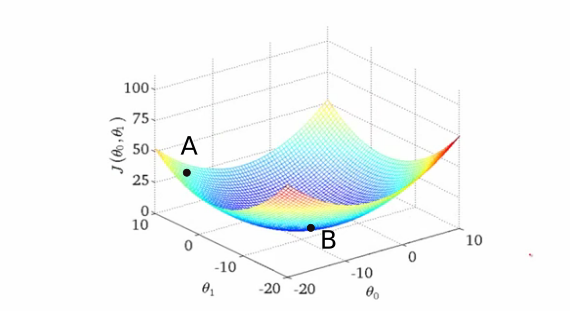
\includegraphics[width=0.8\textwidth]{Figures/gd.png}
 	\caption{Estructura de la imagen de entrada \\ Fuente:  \href{https://blog.paperspace.com/intro-to-optimization-in-deep-learning-gradient-descent/}{\textit{https://blog.paperspace.com/}}}
	\label{image}
\end{figure}

Dentro de la gradiente de descenso podemos diferenciar 3 variantes de acuerdo al la cantidad de datos que se usan para calcular la gradiente de nuestra función objetivo entre estas variantes tenemos a:\\

\subsubsection{Batch gradient descent}
Esta variante calcula la gradiente de descenso de una función de costo, con respecto a un parámetro $\theta$, \textit{para todo el conjunto de datos}. En la ecuación 4.1 podemos observar la actualización que se dará para cada ejecución. $\eta$ representa la tasa o tamaño de los pasos para encontrar el mínimo local.
\begin{equation}
\label{bgds}
\begin{aligned}
\theta &= \theta - \eta \nabla_{\theta} J(\theta)
\end{aligned}
\end{equation}
La ecuación 4.1 asegura la convergencia para mínimo global en una superficie convexa y mínimo local para una superficie no convexa. Entre las dificultades de este método tenemos que puede llegar a ser lento y que esta limitado por la cantidad de datos, ya que esta puede superar a la memoria nuestro computador.	
\subsubsection{Stochastic gradient descent}
Otra variante es \textit{Stochastic gradient descent} que a diferencia del método anterior, realiza las actualizaciones para cada ejemplo de entrenamiento de $(x^{i},y^{i})$ de esta forma se evitan problemas como la generación de redundancia debido a que se realiza una actualización por cada ejemplo de entrenamiento.
\begin{equation}
\label{sgds}
\begin{aligned}
\theta &= \theta - \eta \nabla_{\theta} J(\theta,x^{i},y^{i})
\end{aligned}
\end{equation}
En la figura 4.4 vemos que la función de costo usando SGD fluctúa demasiado esto podría representar un problema pero por el contrario, esta figura representa que el método SGD es capaz de saltar de un mínimo local a otro. Esto permite encontrar mínimos locales potencialmente mejores.

\begin{figure}[H]
	\centering
	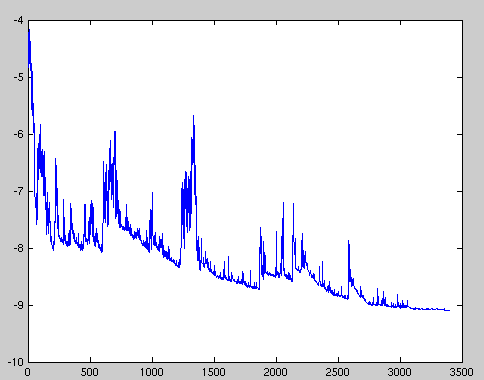
\includegraphics[width=0.5\textwidth]{Figures/sgd.png}
	\caption{Función costo en SGD \\ Fuente:  \href{https://www.doc.ic.ac.uk/~js4416/163/website/neural-networks/optimisers.html}{\textit{www.doc.ic.ac.uk}}}
	\label{funcion costo}
\end{figure} 

\subsubsection{Mini-batch gradient descent}
Este método pude verse como una mezcla de los 2 métodos anteriores, en lugar de aplicarlo para un conjunto entero de datos, los datos se dividen en pequeños conjuntos o mini batches, estos conjunto alimentan nuestro modelo de nuestra red.\\			
Este método nos permite reducir la varianza de las actualizaciones de los parámetros lo cual nos permite una convergencia más estable. El tamaño de los mini-batches oscilan entre 50-250 y varían de acuerdo a su aplicación.

\begin{equation}
\label{mbgds}
\begin{aligned}
\theta &= \theta - \eta \nabla_{\theta} J(\theta,x^{i:i+n},y^{i:i+n})
\end{aligned}
\end{equation}

Mini-batch gradient descent es necesario elegir un $\nabla$ adecuado. Debido  que uno pequeño puede ocasionar una convergencia lenta y una grande puede ocasionar que la fluctué entre los valores mínimos y no converga.\\
Una de sus ventajas principales es que aprovecha el rendimiento de las GPUs para realizar cálculos más rápidos, esto se debe a que la información se guarda como tensores(Matrices de gran dimensión) y las GPUs realizan cálculos de operaciones de matrices más rápidos que una CPU. Es común encontrar a este en otras lecturas como \textit{Stochastic gradient descent} sin realizar distinción alguna del método anteriormente descrito.

\subsection{Optimizadores}
En esta sección analizaremos y entenderemos como funcionan algunos optimizadores en el proceso de mejorar la convergencia de la gradiente de descenso.
\subsubsection{Momentum}
Las SGD tienen problemas para desplazarse en áreas con donde la superficie se curva más en una dimensión que en otra, estos lugares son los alrededores de los óptimos locales. En este escenario la SGD oscilará en la curvatura y descenderá lentamente hacia el óptimo como se muestra en la figura 4.5.
\begin{figure}[H]
	\centering
	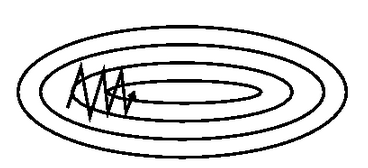
\includegraphics[width=0.5\textwidth]{Figures/momentum1.png}
	\caption{Actualización sin momentum \\ Fuente:  \href{https://www.doc.ic.ac.uk/~js4416/163/website/neural-networks/optimisers.html}{\textit{www.doc.ic.ac.uk}}}
	\label{momentum1}
\end{figure}
El momentum es un método que ayuda a la SGD a acelerar en la dirección correcta, mientras evitas las oscilaciones. El momentum lográ esto añadiendo una fracción $\gamma$ del vector de actualización pasado a nuestro vector presente tal como se muestra en las ecuaciones 4.4.\\ Un valor comúnmente elegido es $\gamma =0.9 $, en las actualización el valor del momentum aumenta para dimensiones cuyos gradientes apuntan en la misma dirección y disminuye para dimensiones en la que la gradiente cambia de dirección. Esto nos asegura que tendremos una convergencia más rápida con una oscilación reducida.En la figura 4.6 se observa gráficamente la aceleración de la convergencia en la SGD.

\begin{equation}
\label{mbgds}
\begin{aligned}
\nu_{t}&=\gamma \nu_{t-1} +  \eta \nabla_{\theta} J(\theta)\\
\theta &= \theta -\nu_{t}
\end{aligned}
\end{equation}

\begin{figure}[H]
	\centering
	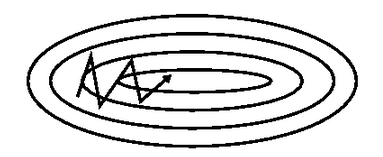
\includegraphics[width=0.5\textwidth]{Figures/momentum2.png}
	\caption{Actualización con momentum \\ Fuente:  \href{https://www.doc.ic.ac.uk/~js4416/163/website/neural-networks/optimisers.html}{\textit{www.doc.ic.ac.uk}}}
	\label{momentum2 }
\end{figure}

\subsubsection{Nesterov accelerated gradient (NAG)}
Este método permite que nuestro descenso sea más controlado, ya que reduce la velocidad antes de volver a subir una pendiente en nuestra superficie de la función de costo. Esta técnica es una variante de momentum donde se usa el término $\gamma \nu_{t-1}$ para mover los parámetros de $\theta$. Al calcular el valor de $\theta - \gamma \nu_{t-1}$ nos permite tener una aproximación de donde se encontrá la siguiente posición de los parámetros. Por lo tanto no calculamos la gradiente en el parámetro $\theta$ actual sino que se calcula en una posición futura aproximada.




\begin{equation}
\label{mbgds}
\begin{aligned}
\nu_{t}&=\gamma \nu_{t-1} + \eta \nabla_{\theta} J(\theta- \gamma \nu_{t-1})\\
\theta &= \theta -\nu_{t}
\end{aligned}
\end{equation}

En la figura 4.7 observamos el proceso. Primero el momentum calcula la gradiente actual(vector azul pequeño)  y luego da un gran salto en la dirección de la gradiente actualizada acumulada (gran vector azul), el NAG primero realiza un gran salto en dirección del gradiente acumulado previo(vector marrón), luego realiza un corrección(vector rojo), esto nos da como resultado la actualización completa de NAG(vector verde). Este calculo anticipado es muy importante debido a que nos impide ir demasiado rápido y mejora la capacidad de respuesta lo cual aumenta el rendimiento de las CNN.
\begin{figure}[H]
	\centering
	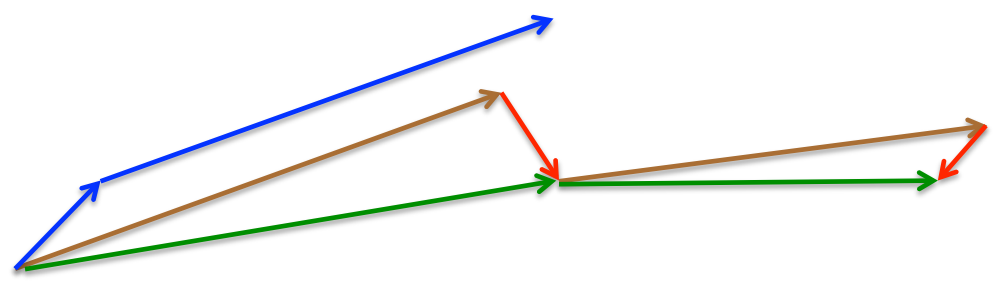
\includegraphics[width=0.5\textwidth]{Figures/nesterov.png}
	\caption{Convergencia Nesterov\\ Fuente:  \href{https://www.doc.ic.ac.uk/~js4416/163/website/neural-networks/optimisers.html}{\textit{www.doc.ic.ac.uk}}}
	\label{nesterov }
\end{figure}
\subsubsection{Adagrad}
Es un algoritmo optimización basado en la gradiente de descenso, este adapta la tasa de aprendizaje. A este tipo de método se les conoce como \textit{adaptativos}. Adagrad realiza actualizaciones más pequeñas para parámetros con características que se repiten con más frecuencia y una tasa alta  para parámetros con características pocas frecuentes. Este método mejor en gran forma nuestra SGD, entre sus ventajas tenemos que es usado para entrenar redes neuronales a gran escala.


En métodos anteriores se usaba la actualización de todos los parámetros $\theta$ al mismo tiempo esto debido a que se usaba la misma tasa de aprendizaje $\eta $. Adagrad usa una tasa de aprendizaje diferente para cada parámetro $\theta_{i}$ en cada paso de tiempo $t$.
En la ecuación 4.6 mostramos los cálculos de la gradiente en un tiempo t.
\begin{equation}
\label{adagrad1}
\begin{aligned}
g_{t,i}&=\nabla_{\theta} J(\theta_{t,i})\\
\theta_{t+1,i} &= \theta_{t,i} -\eta \cdot g_{t,i}
\end{aligned}
\end{equation}
El termino $\cdot g_{t,i}$ representa el valor de la gradiente en el paso de tiempo $t$, el cual es la derivada de la función objetivo con respecto al termino $\theta_{i}$.

Adagrad modifica la idea de utilizar una tasa $\eta$ fija, podemos observar el la ecuación 4.7 es una variante de la ecuación 4.6. En donde se modifica la tasa de aprendizaje en cada paso de tiempo $t$ para todos los parámetros $\theta_{i} $ basándonos en los valores de las gradientes pasadas que fueron calculas para $\theta_{i}$
\begin{equation}
\label{adagrad2}
\begin{aligned}
\theta_{t+1,i} &= \theta_{t,i} - \frac{\eta}{\sqrt{G_{t,ii}+\epsilon}} \cdot g_{t,i}
\end{aligned}
\end{equation}

\begin{itemize}
	\item $G_{t,ii}$: representa la suma de los cuadrados de las gradientes pasadas con respecto a $\theta_{i}$
	\item $\epsilon $ es un término pequeño para evitar la división por 0. $\epsilon$ encuentra en el orden de $10^{-8}$.
\end{itemize}
Como $G_{t} \in \Re^{dxd} $contiene la suma de los cuadrados de las gradientes pasados con respecto a todos los parámetros de $\theta$ a lo largo de la diagonal de su matriz. Esto permite que se pueda realizar el producto matriz-vector.
\begin{equation}
\label{adagrad3}
\begin{aligned}
\theta_{t+1,i} &= \theta_{t,i} - \frac{\eta}{\sqrt{G_{t}+\epsilon}} \odot g_{t,i}
\end{aligned}
\end{equation}
El método Adagrap en palabras de sus autores:
\textquotedblleft Informalmente nuestros procedimientos dan a las características más frecuentes tasas de aprendizaje bajas y para características poco frecuentes tasas de aprendizaje altas. Por lo tanto, la adaptación permite identificar características predictivas pero comparativamente raras. \textquoteright  \cite{ADA} 

De esta afirmación notamos que el principal beneficio de Adagrad es que nos evita el hecho de trabajar con una tasa fija por otro lado su principal desventaja se basa en el la suma de los gradientes al cuadrado aumentará en cada iteración lo cual provocará que su tasa sea cada vez más pequeña.


\subsubsection{RMSprop}
Es un método de aprendizaje por adaptación de la tasa que fue propuesto por Geoff Hinton.
Este modelo se desarrollo con el objetivo resolver el problema de disminuir radicalmente la tasa de aprendizaje en Adagrad.\\ RMSprop divide la tasa de aprendizaje mediante el decaimiento del promedio de la suma de las gradientes al cuadrado.
\begin{equation}
\label{RMS}
\begin{aligned}
E[g^2]_{t} &= \gamma E[g^2]_{t-1} + (1-\gamma)g^{2}_{t}\\
\theta_{t+1} &= \theta_{t} - \frac{\eta}{\sqrt{E[g^2]_{t} +\epsilon }} g_{t}
\end{aligned}
\end{equation}
\begin{itemize}
	\item $E[g^2]$: Promedio de la raíz de nuestro gradiente en cada peso.
	\item $\gamma$  : Parámetro de decaimiento
	\item $\eta$    : Tasa de aprendizaje
\end{itemize}
Divide la gradiente $g_{t}$ por la raíz $\sqrt{E[g^2]_{t} +\epsilon}$ hace que el aprendizaje trabaje mucho mejor.
\subsubsection{Adam	}
Adam es un algoritmo de optimización que desarrollado por Diederik Kingma y Jimmy ba\cite{ADAM} .
Adaptative moment estimation  o Adam, calcula una tasa de aprendizaje adaptativo para cada parámetro. Este método mantiene un decaimiento exponencial del promedio de las gradientes anteriores. El método tiene refiere los mínimos en las superficies de error.
 En la ecuación 4.10 mostramos el cálculo del promedio de decaimiento de las gradientes pasadas $m_{t}$ y el cuadrado de las gradientes pasadas $v_{t}$
\begin{equation}
\label{adam1}
\begin{aligned}
m_{t} &= \beta_{1} m_{t-1} +(1-\beta_{1})g_{t} \\
v_{t} &= \beta_{2} v_{t-1} +(1-\beta_{2})g_{t}^2
\end{aligned}
\end{equation}

\begin{itemize}
	\item $m_{t}:$ Primer momento (media)
	\item $v_{t}:$ Segundo momento de la gradiente
	\item $\beta_{1}:$ Taza de decaimiento del primer momento.
	\item $\beta_{2}:$ Taza de decaimiento del segundo momento.
\end{itemize}
En la ecuación 4.11 mostramos la forma de calcular estimado de la primer y segundo momento.
\begin{equation}
\label{adam2}
\begin{aligned}
\hat{m_{t}}&= \frac{m_{t}}{1-\beta_{1}^{t}} \\
\hat{v_{t}} &= \frac{v_{t}}{1-\beta_{2}^{t}}
\end{aligned}
\end{equation}

\begin{itemize}
	\item $\hat{m_{t}}:$ Estimación del Primer momento (media)
	\item $\hat{v_{t}}:$ Estimación del Segundo momento de la gradiente.
\end{itemize}

La ecuación 4.12 muestra la regla de actualización en Adam. Se utiliza el $\epsilon$ para prevenir una división por cero.
\begin{equation}
\label{adam3}
\begin{aligned}
\theta_{t+1}&= \theta_{t+1} - \frac{\eta}{\sqrt{\hat{v_{t}}}+\epsilon} \hat{m_{t}}	
\end{aligned}
\end{equation}

